\subsection{Smoothed Particle Hydrodynamics}


\subsection{Miluphcuda SPH code}
Miluphcuda is a GPU accelerated smoothed particle hydrodynamics code that has been developed over several years at the University of Tuebingen by Christoph Schaefer and others. Its general use is well documented in \cite{Schaefer_2016}.

\subsubsection{Porosity model}
The model used is based upon the
\subsubsection{Strength model}

\subsubsection{Variable smoothing length
}


\subsubsection{Time Integration}
1) Timestep algorithm for velocity update (RungeKutta 2)
2) Update particle positions from velocity and acceleration (accel from Navier Stokes)
3) Error criterium for timestep (what is used? RK45?)

- how are the equations from Theory section used to get the development over time
- final form of Equation we used:
.........................
- Neighborhoudsearch instead of computing Kernel over all particles is faster
- Upper limit to maximum neighbor particles

\subsection{Initial conditions}
- resolution bound to variable smoothing length
- SPH needs uniform macro structure but random micro structure


\begin{figure}
    \centering
    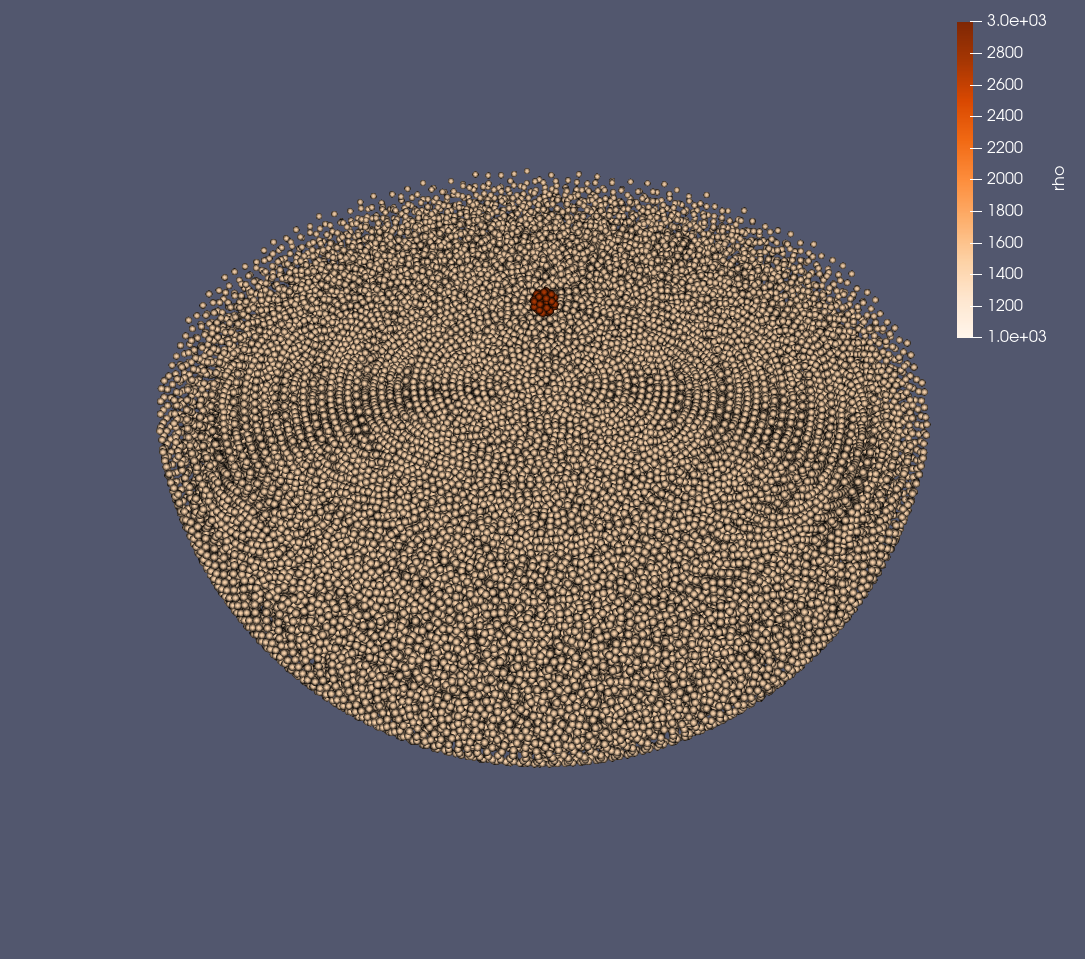
\includegraphics[width=\textwidth]{impact_start.png}
    \caption{initial conditions}
    \label{fig:impact_start}
\end{figure}

\begin{figure}
    \centering
    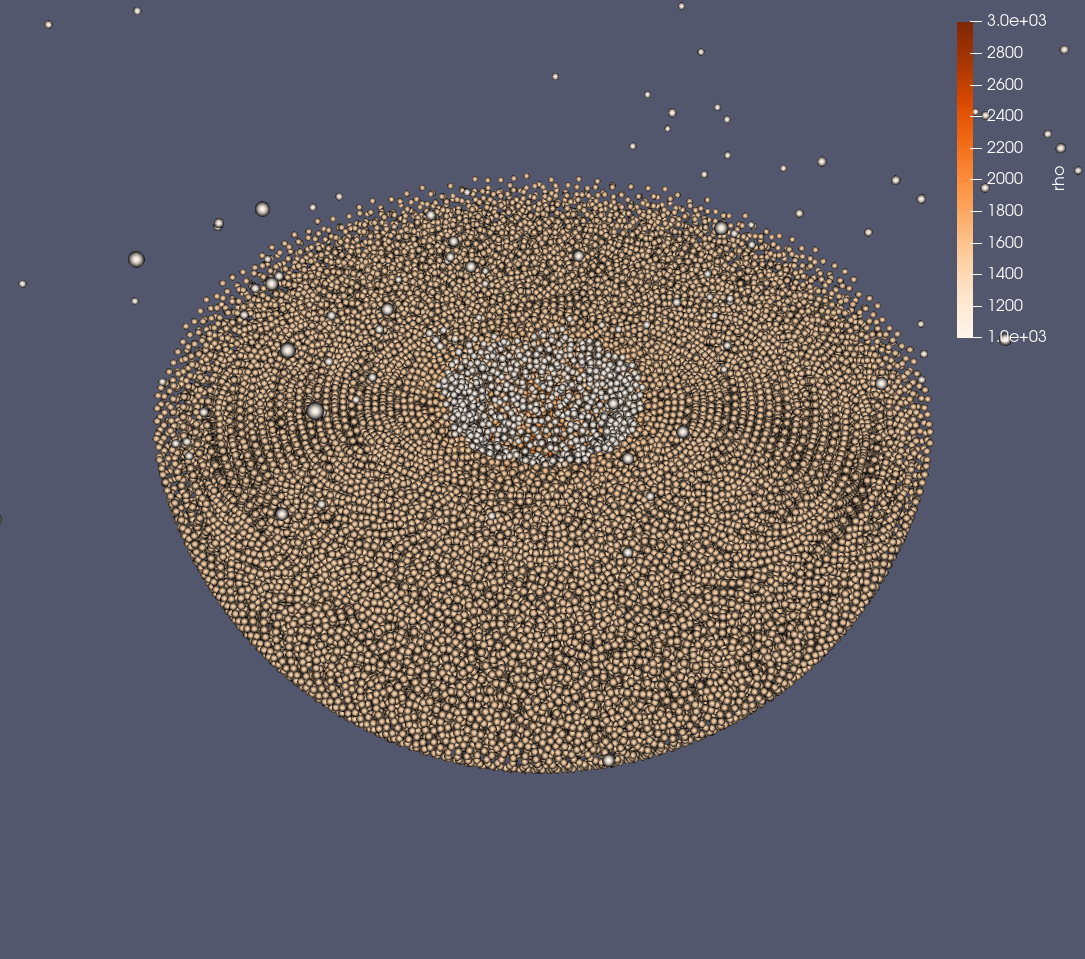
\includegraphics[width=\textwidth]{impact_end.png}
    \caption{cratering of half sphere}
    \label{fig:impact_end}
\end{figure}




